%==============================================================================
%  Tesis — Maestría en Economía Aplicada (ITAM)
%  Andamio LaTeX reutilizado de la tesina de licenciatura del autor.
%  Documento de trabajo: reemplaza la versión de 2024 (Paper_Inv_Aplicada_II).
%==============================================================================

\documentclass[11pt, oneside]{book}

\usepackage[utf8]{inputenc}
\usepackage[spanish]{babel}
\addto\captionsspanish{\renewcommand{\tablename}{Tabla}}

\usepackage{amssymb,amsmath,amsthm}
\usepackage{bbm}
\usepackage{graphicx}
\usepackage{float}
\usepackage{booktabs}
\usepackage{longtable}
\usepackage{multirow}
\usepackage[table,xcdraw]{xcolor}
\usepackage{colortbl}
\usepackage{pdflscape}
\usepackage{tabularx}
\usepackage{adjustbox}
\usepackage{enumerate}
\usepackage{subcaption}
\usepackage{natbib}
\usepackage{hyperref}

\usepackage[paperwidth=17cm, paperheight=22.5cm, bottom=2.5cm, right=2.5cm]{geometry}

\graphicspath{{imagenes/}}

% Formato heredado de la tesina
\tolerance=1
\emergencystretch=\maxdimen
\hyphenpenalty=10000
\hbadness=10000
\linespread{1.25}

\usepackage[justification=centering, font=bf, labelsep=period, skip=5pt]{caption}
\newcommand{\imagesource}[1]{{\footnotesize Fuente: #1}}

\definecolor{mycitecolor}{RGB}{0,0,255}
\hypersetup{
  colorlinks=true,
  linkcolor=mycitecolor,
  citecolor=mycitecolor,
  urlcolor=black,
}

\begin{document}

%------------------------------------------------------------------------------
%  PORTADA
%------------------------------------------------------------------------------
\begin{titlepage}
\begin{center}

\textsc{\Large Instituto Tecnológico Autónomo de México}\\[2em]

\begin{figure}[h]
\begin{center}

\includegraphics[scale=0.50]{itam_logo.png}
\end{center}
\end{figure}

\textbf{\LARGE EL EFECTO DE LAS MULTAS SOBRE LOS ACCIDENTES DE TRÁFICO}\\[2em]
% TODO: revisar título a la luz del rediseño (enforcement / renovación 2022 / víctimas)

\textsc{\large Tesis}\\[1em]
\textsc{\large que para obtener el grado de}\\[1em]
\textsc{\LARGE Maestro en Economía Aplicada}\\[1em]
\textsc{\large Presenta}\\[1em]
\textsc{\LARGE Luis Fernando Hernández Mendoza}\\[1em]
\textsc{\large Asesor}\\[1em]
\textsc{\LARGE Dr. Horacio Alejandro Larreguy Arbesú}\\[2em]

\end{center}
\vspace*{\fill}
\textsc{Ciudad de México \hspace*{\fill} 2026}
\end{titlepage}

%------------------------------------------------------------------------------
%  DECLARACIÓN
%------------------------------------------------------------------------------
\thispagestyle{empty}
\vspace*{\fill}
\begingroup
\noindent
«Con fundamento en los artículos 21 y 27 de la Ley Federal del Derecho de Autor
y como titular de los derechos moral y patrimonial de la obra titulada
``\textbf{El efecto de las multas sobre los accidentes de tráfico}'', otorgo de
manera gratuita y permanente al Instituto Tecnológico Autónomo de México y a la
Biblioteca Raúl Bailléres Jr., la autorización para que fijen la obra en
cualquier medio, incluido el electrónico, y la divulguen entre sus usuarios,
profesores, estudiantes o terceras personas, sin que pueda percibir por tal
divulgación una contraprestación.»

\centering
\vspace{5em}
\rule[1em]{20em}{0.5pt}\\ \textsc{Fecha}
\vspace{8em}
\rule[1em]{20em}{0.5pt}\\ \textsc{Luis Fernando Hernández Mendoza}
\endgroup
\vspace*{\fill}

%------------------------------------------------------------------------------
%  FRONTMATTER
%------------------------------------------------------------------------------
\pagestyle{plain}
\frontmatter

\chapter*{Agradecimientos}
% TODO

\chapter*{Resumen}
\noindent
Evalúo si el aumento de la fiscalización vial asociado a la renovación de la
Policía de Tránsito de la Ciudad de México (abril de 2022) redujo las víctimas
de hechos de tránsito. Construyo un panel colonia-mes de 1{,}814 unidades
territoriales y defino el tratamiento como la exposición espacial —por
\emph{buffers} de 250 a 1{,}500 metros— a la infraestructura de radares fijos
y móviles vigente el año previo al evento. Comparo la evolución de las
colonias expuestas y no expuestas mediante un estudio de evento con efectos
fijos de colonia y de mes, usando como \emph{outcome} principal las víctimas
de hechos de tránsito registradas por la Fiscalía General de Justicia y, como
evidencia de que la reforma efectivamente incrementó la fiscalización, las
infracciones emitidas cerca de esa misma infraestructura.

No encuentro evidencia robusta de un efecto sobre las víctimas. Las víctimas
fallecidas —el \emph{outcome} menos sensible a la probabilidad de que un
hecho se registre formalmente— no se mueven en ninguna especificación, y el
aumento aparente en víctimas totales bajo mínimos cuadrados (12 a 21\,\%) no
sobrevive a un modelo de conteo Poisson, que es la especificación
econométricamente apropiada dado que el 89\,\% de las observaciones del panel
son ceros. El resultado se replica, con el mismo patrón, en un segundo evento
de política vial (septiembre de 2023). El primer paso del mecanismo —el
incremento en infracciones cerca de la infraestructura de fiscalización— es
en sí mismo débil y transitorio, por lo que interpreto el nulo como ausencia
de evidencia de un efecto bajo un tratamiento de fiscalización diferencial
débil, más que como una estimación precisa de un efecto verdaderamente cero.

\tableofcontents
\listoftables
\listoffigures

%------------------------------------------------------------------------------
%  CUERPO
%------------------------------------------------------------------------------
\mainmatter
\pagestyle{plain}

\chapter*{Introducción}
\addcontentsline{toc}{chapter}{Introducción}

% ==========================================================================
% BASE: introducción de la versión 2024 (Paper_Inv_Aplicada_II, pp. 1-3).
% AJUSTES:
%  - El objeto ya no es "el efecto de las multas" en abstracto sino la
%    evaluación de un cambio de política concreto (renovación de la Policía de
%    Tránsito, abril 2022) y su fiscalización diferencial en el espacio.
%  - Anticipar el resultado nulo y su lectura (ausencia de evidencia en un
%    contexto de tratamiento débil), no un hallazgo de "las multas aumentan
%    los accidentes".
%  - Mencionar la nueva fuente de víctimas (FGJ) y la unidad colonia-mes.
% ==========================================================================

\noindent
% --- Párrafo 1: relevancia (reutilizable de 2024) ---
La seguridad vial es un tema central de la política pública a nivel global. De
acuerdo con la Organización Mundial de la Salud, cada año fallecen alrededor de
1.3 millones de personas por hechos de tránsito y decenas de millones más
resultan lesionadas, con costos económicos asociados a la atención médica, la
pérdida de productividad y los daños materiales.

% --- Párrafo 2: la fiscalización como herramienta ---
La imposición de multas por infracciones de tránsito —exceso de velocidad,
conducción bajo los efectos del alcohol, no uso del cinturón— es una de las
herramientas más utilizadas para inducir el cumplimiento de las normas y
disuadir los comportamientos de riesgo. La evidencia sobre su efectividad, sin
embargo, es mixta y sensible al contexto (Capítulo~\ref{chap:literatura}).

% --- Párrafo 3: la pregunta de esta tesis ---
Esta tesis evalúa si el aumento de la fiscalización vial asociado a la
\textbf{renovación de la Policía de Tránsito de la Ciudad de México de abril de
2022} redujo las víctimas de hechos de tránsito. La estrategia explota la
\emph{aplicación diferencial en el espacio} de la reforma: se comparan las
colonias expuestas a la infraestructura de fiscalización preexistente con las no
expuestas, antes y después del cambio, con datos a nivel colonia-mes.

% --- Párrafo 4: qué se encuentra (adelanto) ---
% TODO redactar con cuidado. Borrador:
No se encuentra evidencia robusta de un efecto sobre las víctimas. Las víctimas
fallecidas no cambian; el aumento aparente en las víctimas totales no sobrevive
a un modelo de conteo y coincide con un repunte transitorio de las multas, lo
que apunta a un efecto de reporte. La fiscalización diferencial que induce la
reforma es, además, débil y de corta duración.

% --- Párrafo 5: estructura del documento (reutilizable, actualizar refs) ---
El documento se organiza como sigue. El Capítulo~\ref{chap:literatura} revisa la
literatura sobre fiscalización y seguridad vial. El Capítulo~\ref{sec:contexto}
describe el contexto de la política vial en la Ciudad de México y la reforma de
2022. El Capítulo~\ref{chap:datos} presenta las fuentes y las variables. El
Capítulo~\ref{chap:estrategia} define la estrategia empírica. El
Capítulo~\ref{chap:resultados} presenta los resultados y la robustez. El
Capítulo~\ref{chap:conclusiones} concluye.

\chapter{Revisión de literatura}
\label{chap:literatura}

\noindent
La relación entre fiscalización de tránsito y siniestralidad ha sido estudiada
desde perspectivas y contextos diversos, con resultados heterogéneos. Esta
tesis se sitúa en la intersección de dos literaturas: la que relaciona el
volumen de multas con la siniestralidad, y la más amplia —y más cercana al
diseño de este trabajo— sobre disuasión (\emph{deterrence}) a través de la
presencia y capacidad de fiscalización de la autoridad.

\section{Multas y siniestralidad}

Varios trabajos documentan una asociación positiva entre historial de
infracciones y riesgo de siniestro a nivel individual. \citet{factor2014}
encuentra, con regresiones logísticas sobre datos de Israel, que quienes han
recibido multas en el pasado son más propensos a sufrir hechos de tránsito.
\citet{huajing2022} halla, para la provincia de Anhui, que conductas como el
exceso de velocidad y la conducción distraída se asocian a mayor riesgo de
siniestros fatales.

En el plano causal, \citet{luca2015} usa un diseño de variables instrumentales a
partir del programa ``Click-it-or-Ticket'' en Massachusetts y concluye que las
multas ayudan a generar conciencia entre los conductores. \citet{makowsky2011}
encuentran, para municipios de Estados Unidos con restricciones
presupuestales, que un mayor volumen de multas se asocia con menos siniestros.
\citet{mphela2013} reporta, para Botswana, que el efecto de la aplicación de la
ley sobre las muertes viales es limitado, y sugiere que elevar la edad mínima
para obtener licencia podría ser más efectivo que endurecer las sanciones
económicas.

\section{Enforcement policial y disuasión}

Un cuerpo distinto de literatura —más cercano al diseño de esta tesis— no mide
el efecto de la multa individual, sino el de la \emph{capacidad de
fiscalización} de la autoridad, sea esta medida en agentes, patrullas u
operativos. El marco teórico de referencia es \citet{becker1968}: la
probabilidad percibida de ser sancionado, y no solo la severidad de la
sanción, es lo que determina el efecto disuasivo sobre el comportamiento. Esta
distinción es relevante para esta tesis porque el diseño empírico evalúa un
cambio en la \emph{capacidad de fiscalización} (número y digitalización de
agentes autorizados para infraccionar) más que en el monto de las multas.

La evidencia empírica más cercana a este trabajo es \citet{deangelohansen2014},
quienes explotan un recorte presupuestal que redujo en 35\,\% el número de
oficiales de la patrulla carretera de Oregón en 2003. Encuentran que la caída
en infracciones emitidas estuvo acompañada de un aumento significativo en
lesiones y muertes viales, y estiman que cada \$309{,}000 dólares de gasto
adicional en patrullaje carretero previene una muerte vial. El diseño de
\citeauthor{deangelohansen2014} es, en esencia, el espejo del de esta
tesis: en vez de una reducción de agentes, aquí se explota un aumento
diferencial en la capacidad de fiscalización, y en vez de variación temporal
pura, se explota variación espacial en la exposición a la infraestructura de
fiscalización. \citet{chalfinmccrary2017}, en una revisión exhaustiva de la
literatura de disuasión criminal, documentan un patrón consistente con este
resultado: existe evidencia sólida de que el comportamiento responde a la
presencia y capacidad de la policía, pero mucho menos evidencia de que
responda a la severidad de la sanción en sí misma —una distinción que motiva
tratar las multas como \emph{mecanismo} y no como la variable de interés
central de este trabajo (Sección~\ref{sec:estrategia_outcomes}).

\section{Evidencia para la Ciudad de México}

La referencia local más cercana a esta tesis es \citet{quintero2023}, quienes
evalúan mediante un diseño de series de tiempo interrumpido controlado (CITS)
un conjunto de políticas de seguridad vial de la Ciudad de México entre 2015 y
2019. Encuentran resultados opuestos según el tipo de sanción: las políticas
de 2015 —métodos automáticos de detección de exceso de velocidad, uso del
celular o giros prohibidos, con consecuencia económica directa (fotomultas)—
se asocian a una \emph{disminución} de la mortalidad vial, mientras que la
política de 2019 —el sistema de puntos sin consecuencia económica inmediata
(Fotocívicas, Sección~\ref{sec:contexto_politica})— se asocia a un
\emph{incremento}. Este hallazgo es un antecedente directo para esta tesis:
sugiere que la naturaleza de la sanción (económica vs. administrativa) importa
tanto como su volumen, y anticipa que el vínculo entre más fiscalización y
menos víctimas no es automático en el contexto específico de la Ciudad de
México.

\section{Aporte de esta tesis}

Esta tesis se distingue de la literatura revisada en tres puntos. Primero, la
mayoría de la evidencia sobre multas y siniestralidad —incluida la versión
2024 de este mismo proyecto— se concentra en el volumen de infracciones como
variable de interés y trata a la policía como un agente pasivo que solo
multa; aquí, siguiendo más de cerca a \citet{deangelohansen2014}, el objeto de
estudio es un cambio institucional en la capacidad de fiscalización, y las
multas se usan únicamente como evidencia de que ese cambio se tradujo en más
actividad de enforcement. Segundo, la evidencia para América Latina y, en
particular, para unidades espaciales finas dentro de una misma ciudad es
escasa: \citet{quintero2023} evalúa políticas a nivel ciudad; este trabajo
explota variación \emph{dentro} de la Ciudad de México mediante exposición
espacial a la infraestructura de fiscalización. Tercero, esta tesis pone
atención explícita a los efectos de reporte en los datos administrativos de
víctimas —una amenaza a la identificación que rara vez se discute
formalmente en esta literatura— al usar fallecidos, un desenlace mucho menos
sensible a la probabilidad de que un hecho se registre formalmente, como
verificación de robustez del resultado principal
(Sección~\ref{sec:contexto_espacial} y capítulo~\ref{chap:resultados}).

\chapter{Contexto}
\label{sec:contexto}

\section{La política de fiscalización vial en la Ciudad de México}
\label{sec:contexto_politica}

En abril de 2019 la Ciudad de México sustituyó el esquema de fotomultas —una
sanción puramente económica por exceso de velocidad captada por cámara— por el
sistema Fotocívicas, en el que la infracción se traduce en la pérdida de
puntos sobre la licencia de conducir y solo de forma secundaria en una multa
monetaria. El cambio es relevante para esta tesis porque altera el incentivo
que enfrenta el conductor: \citet{quintero2023}, en un análisis de series de
tiempo interrumpido para la Ciudad de México, documentan que las políticas de
tránsito con consecuencia económica directa (2015) se asociaron a una
reducción de la mortalidad vial, mientras que el sistema de puntos sin costo
económico inmediato (2019) se asoció más bien a un incremento. Este
antecedente anticipa que el vínculo entre fiscalización y víctimas no es
mecánico, y es consistente con el resultado nulo que se documenta en el
capítulo~\ref{chap:resultados}.

La infraestructura física de fiscalización —radares fijos y móviles que
alimentan Fotocívicas— se mantuvo relativamente estable en el periodo de
estudio: pasó de 116 dispositivos en 2019 (89 fijos y 27 móviles) a 109 en
2020 y 2021, 105 en 2022 y 121 en 2023, con una composición dominada en todos
los años por los radares fijos (entre 79 y 103 unidades). El diseño empírico
de esta tesis usa como definición del \emph{tratamiento} el inventario de
2021 —91 radares fijos y 18 móviles, geolocalizados— por ser el más cercano y
predeterminado respecto al evento principal (sección~\ref{sec:eventos}).

Sobre esta infraestructura relativamente estable se superponen cambios en
\emph{quién} puede infraccionar y \emph{cómo}. En febrero de 2021 se
modificaron las facultades de infracción de los agentes de tránsito. El
cambio de mayor relevancia para esta tesis ocurrió en abril de 2022, cuando
la Secretaría de Seguridad Ciudadana puso en marcha el Programa de Renovación
de la Policía de Tránsito \citep{elfinanciero2022}. El programa sustituyó a
la generalidad de policías preventivos —que hasta entonces podían
infraccionar— por un cuerpo reducido y especializado (100 elementos en su
arranque), identificados con un brazalete y obligados a levantar cada
infracción con un dispositivo electrónico y aplicación móvil, en vez del
talonario físico. En el mismo periodo entró en vigor un nuevo reglamento de
tránsito que, en paralelo, redujo el número de oficiales autorizados para
infraccionar y acotó los motivos por los que un vehículo puede ser remitido
al corralón \citep{galvan2022}. Ambos cambios describen la misma reforma
desde ángulos distintos: menos agentes, pero con mayor capacidad de
fiscalización efectiva por agente al estar digitalizados y ser trazables.
Es esta reforma —no el reglamento de 2022 como choque homogéneo citywide— la
que se usa como evento en el diseño empírico, precisamente porque su
implementación fue gradual y territorialmente desigual, lo que genera
variación explotable entre colonias.

Un tercer momento relevante es septiembre de 2023, cuando entró en vigor una
reforma dirigida específicamente a motociclistas (uso obligatorio de
aditamentos luminosos, visor y chamarra o peto de protección), tras un
periodo de intensificación de operativos que comenzó en enero de ese año.
Esta reforma se evalúa como evento candidato en la
sección~\ref{sec:eventos} y se usa como replicación de robustez en el
capítulo~\ref{chap:resultados}, aunque finalmente no es el evento principal
por las razones que se detallan ahí.

\section{Evolución de la siniestralidad}
\label{sec:contexto_siniestralidad}

La figura~\ref{fig:serie_victimas} muestra la serie mensual de víctimas de
hechos de tránsito registradas por la Fiscalía General de Justicia de la
Ciudad de México (FGJ CDMX) entre enero de 2019 —primer mes con cobertura
sistemática en los registros— y julio de 2024. Se observan tres rasgos
relevantes para el diseño empírico. Primero, la caída de movilidad asociada a
la pandemia de COVID-19 se refleja en un mínimo de víctimas hacia mediados de
2020, seguida de una recuperación gradual conforme se normalizó la
movilidad. Segundo, 2022 fue un año particularmente severo: la ciudad
registró 719 víctimas mortales, con los motociclistas como el grupo más
afectado (39\,\% de los fallecidos), seguidos de peatones (29\,\%), pasajeros
(17\,\%), conductores (9\,\%) y ciclistas (5\,\%) \citep{navarrete2023}. Este
repunte es contemporáneo a la renovación de la Policía de Tránsito descrita
en la sección anterior, lo que motiva usar ese evento como referencia
temporal del diseño. Tercero, ni las víctimas totales ni los fallecidos
muestran una caída sostenida después de abril de 2022; si acaso, la
tendencia de mediano plazo es ligeramente ascendente hacia 2023-2024. Esta
observación anticipa, de forma puramente descriptiva, el resultado nulo que
se documenta formalmente en el capítulo~\ref{chap:resultados}.

\begin{figure}[H]
  \centering
  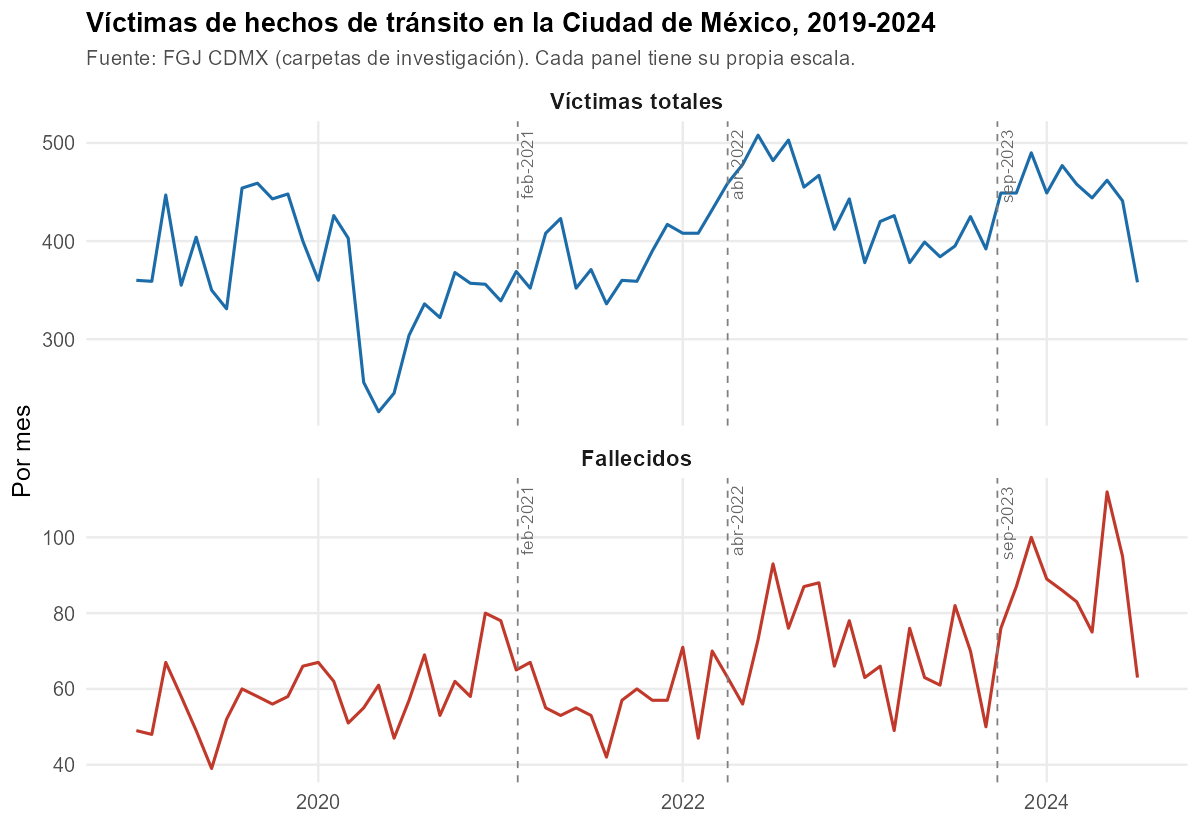
\includegraphics[width=\textwidth]{401_serie_victimas_2019_2024.png}
  \caption{Víctimas de hechos de tránsito en la Ciudad de México, 2019-2024.
  Las líneas verticales marcan los tres eventos candidatos discutidos en la
  sección~\ref{sec:eventos}.}
  \imagesource{elaboración propia con datos de la FGJ CDMX.}
  \label{fig:serie_victimas}
\end{figure}

\section{Distribución espacial de la fiscalización}
\label{sec:contexto_espacial}

El diseño de exposición espacial que se define en el
capítulo~\ref{chap:estrategia} descansa en una asimetría empírica entre
dónde ocurre la fiscalización y dónde ocurren las víctimas. La
figura~\ref{fig:mapa_infracciones} muestra que las infracciones de tránsito
2020-2023 se concentran de forma extrema en un número reducido de colonias
—principalmente corredores viales primarios de Miguel Hidalgo, Cuauhtémoc,
Álvaro Obregón y Venustiano Carranza—: el 10\,\% de las colonias con más
infracciones concentra el 98.8\,\% del total registrado. En contraste, la
figura~\ref{fig:mapa_victimas} muestra que las víctimas de tránsito
2019-2024 se distribuyen de forma considerablemente más homogénea en el
territorio: el mismo umbral del 10\,\% de colonias más afectadas concentra
apenas el 44.3\,\% de las víctimas.

Esta asimetría espacial es, en buena medida, lo que justifica la elección
del diseño empírico: si la fiscalización estuviera distribuida de forma tan
concentrada como las infracciones, casi toda la variación identificante
provendría de un puñado de colonias atípicas. El uso de efectos fijos de
colonia junto con una definición de tratamiento basada en buffers de
distancia a la infraestructura de radares (en vez de, por ejemplo,
infracciones per cápita) busca precisamente evitar que la estimación quede
dominada por esas colonias de muy alta concentración de multas.

\begin{figure}[H]
  \centering
  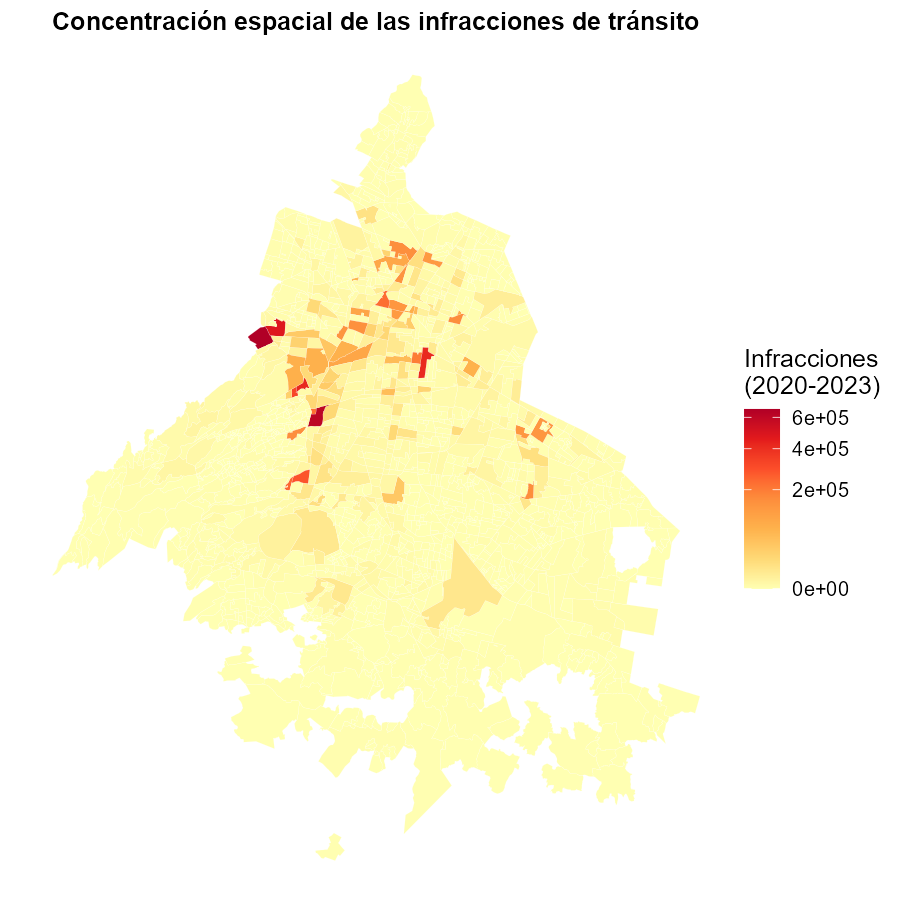
\includegraphics[width=0.85\textwidth]{402_mapa_infracciones_colonia.png}
  \caption{Concentración espacial de las infracciones de tránsito por
  colonia, 2020-2023.}
  \imagesource{elaboración propia con datos de infracciones de tránsito y
  el catálogo de colonias del IECM.}
  \label{fig:mapa_infracciones}
\end{figure}

\begin{figure}[H]
  \centering
  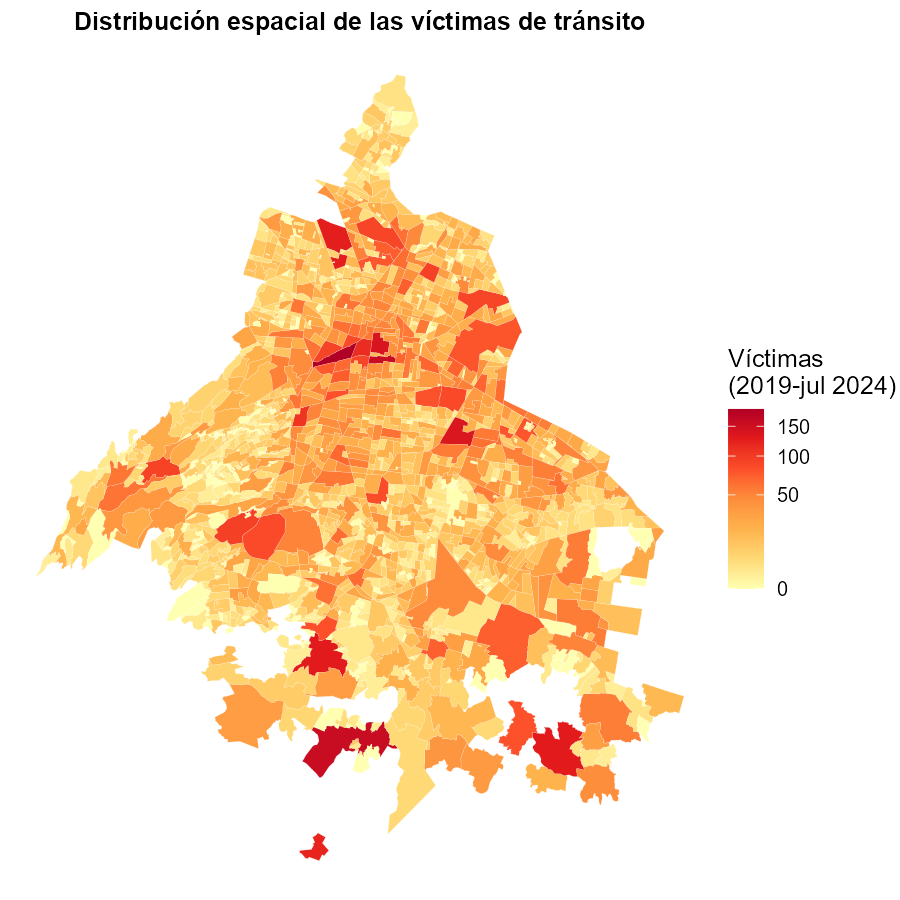
\includegraphics[width=0.85\textwidth]{403_mapa_victimas_colonia.png}
  \caption{Distribución espacial de las víctimas de tránsito por colonia,
  2019-jul 2024.}
  \imagesource{elaboración propia con datos de la FGJ CDMX y el catálogo de
  colonias del IECM.}
  \label{fig:mapa_victimas}
\end{figure}

\section{Eventos candidatos considerados}
\label{sec:eventos}

La línea del tiempo de política vial 2019-2024 ofrece más de un candidato
plausible para un diseño de evento. Se evaluaron tres:

\begin{itemize}
  \item \textbf{Febrero de 2021} — modificación de las facultades de
  infracción de los agentes de tránsito. Se descarta como evento principal
  porque coincide con la fase de recuperación post-COVID de la movilidad, lo
  que hace difícil separar el efecto de la reforma del efecto mecánico de
  más autos en circulación; además, la fiscalización está deprimida en ese
  periodo y el diseño no supera la prueba conjunta de tendencias previas
  (sección~\ref{sec:pretendencias}).
  \item \textbf{Abril de 2022} — renovación de la Policía de Tránsito. Es el
  único de los tres eventos con una primera etapa plausible (más
  fiscalización, aunque débil y transitoria) y con tendencias previas
  válidas para el outcome de víctimas. Se adopta como \textbf{evento
  principal} del diseño.
  \item \textbf{Septiembre de 2023} — reforma dirigida a motociclistas. Se
  descarta como evento principal por dos razones: la cobertura de
  infracciones en los datos administrativos termina en abril de 2023, por lo
  que no hay outcome de mecanismo posterior al evento; y la variación
  espacial de la exposición es más débil que en abril de 2022. Se usa, en
  cambio, como \textbf{replicación de robustez} en el
  capítulo~\ref{chap:resultados}.
\end{itemize}

El capítulo~\ref{chap:estrategia} retoma el evento de abril de 2022 y define
formalmente el tratamiento, la especificación de estudio de evento y los
supuestos de identificación del diseño.

\chapter{Datos y variables}
\label{chap:datos}

% ==========================================================================
% BASE: capítulo 3 de la versión 2024 (pp. 12-16): panel código postal-mes,
% descriptivos, promedios por alcaldía, CP con más infracciones/incidentes.
% AJUSTES:
%  - Unidad: colonia (unidad territorial IECM), no código postal.
%  - Nueva fuente principal de outcome: víctimas FGJ (2019-jul 2024).
%  - Nueva construcción del tratamiento: exposición a radares por buffer.
%  - Documentar la auditoría de la muestra (Horacio: "mejorar construcción y
%    documentación de la muestra").
%  - Documentar los problemas de cobertura de infracciones (abr-jun 2021).
% ==========================================================================

\section{Fuentes}

El \emph{outcome} principal proviene de las carpetas de investigación de la
Fiscalía General de Justicia de la Ciudad de México (FGJ), que registran a
cada persona involucrada en un hecho de tránsito entre enero de 2019 y julio
de 2024. De este universo se conservan únicamente las lesiones y los
homicidios culposos por tránsito vehicular, lo que deja alrededor de
27{,}000 víctimas, de las cuales cerca de 4{,}400 fallecieron; el 88\% de los
registros cuenta con coordenadas propias, y el resto se ubica por coincidencia
de nombre de colonia. Como \emph{outcome} secundario se usa la serie
georreferenciada de incidentes viales reportados a los sistemas de atención de
emergencias del C5, disponible de forma continua desde 2014 hasta febrero de
2024; a diferencia de las víctimas, este registro no distingue gravedad ni
depende de que se abra una carpeta de investigación, por lo que sirve como
punto de comparación frente a un posible efecto de reporte
(Sección~\ref{sec:contexto_espacial}).

El mecanismo del diseño —si la reforma efectivamente incrementó la actividad
de fiscalización— se documenta con la base histórica de infracciones al
Reglamento de Tránsito, que cubre de enero de 2020 a abril de 2023 y en la que
el artículo 9 (exceso de velocidad) concentra por sí solo cerca del 77\% de
los registros. El tratamiento, por su parte, se construye a partir del
inventario anual de radares fijos y móviles y equipos asociados de
Fotocívicas, disponible de 2019 a 2024 y georreferenciado equipo por equipo,
según se describe en la sección siguiente. Todas estas fuentes se agregan
sobre la misma malla territorial: las 1{,}814 unidades del catálogo de
colonias del Instituto Electoral de la Ciudad de México, que es también la
unidad de observación del panel.

\section{Panel colonia-mes}

Se construye un panel balanceado de 1{,}814 colonias por 103 meses (enero de
2016 a julio de 2024). Cada \emph{outcome} se agrega al nivel colonia-mes por
asignación espacial (punto en polígono) o, para las infracciones sin
coordenadas a partir de mayo de 2021, por coincidencia de nombre de colonia.
Cada fuente lleva un indicador de cobertura temporal; fuera de su periodo de
cobertura los conteos se dejan como ausentes, no como cero.

\section{Construcción de la exposición a la infraestructura}
\label{sec:datos_exposicion}

Para cada colonia y cada año entre 2019 y 2024 se calcula, a partir del
inventario georreferenciado de radares fijos y móviles, tres medidas de
exposición: el número de equipos a menos de $b$ metros del polígono de la
colonia, la distancia al equipo más cercano, y la proporción del área de la
colonia que cae dentro de ese radio. Estas tres medidas se calculan para
cuatro definiciones de \emph{buffer} ($b \in \{250, 500, 1000, 1500\}$
metros), y de la primera de ellas se deriva el indicador binario
$\text{tratada}_i(b)$ que se usa como definición principal del tratamiento en
el capítulo~\ref{chap:estrategia}.

El diseño usa el inventario de 2021 —el más cercano y predeterminado respecto
al evento de abril de 2022— para fijar qué colonias cuentan como tratadas. La
tabla~\ref{tab:tratamiento_buffer} muestra que esta definición es, como es de
esperarse, sensible al radio elegido: pasa de 215 colonias tratadas (11.9\,\%
del total) con $b=250$\,m a 837 (46.1\,\%) con $b=1500$\,m. El capítulo de
resultados reporta el efecto para $b \in \{250, 500, 1000\}$ como análisis de
sensibilidad. Vale la pena notar que, aunque el número de radares por año
fluctúa moderadamente (Sección~\ref{sec:contexto_politica}), el conjunto de
colonias tratadas con $b=500$\,m se mantiene relativamente estable entre 2019
y 2024 (16.9\,\% a 20.2\,\%): la infraestructura se reubica poco de un año a
otro, lo que hace razonable fijar el inventario de 2021 como definición de
tratamiento predeterminada al evento.

\begin{table}[H]
  \centering
  \caption{Colonias tratadas por definición de \emph{buffer}, inventario 2021}
  \label{tab:tratamiento_buffer}
  \begin{tabular}{lrrr}
    \toprule
    Buffer & Colonias tratadas & Total & \% tratadas \\
    \midrule
    250 m  & 215 & 1{,}814 & 11.9\,\% \\
    500 m  & 328 & 1{,}814 & 18.1\,\% \\
    1{,}000 m & 590 & 1{,}814 & 32.5\,\% \\
    1{,}500 m & 837 & 1{,}814 & 46.1\,\% \\
    \bottomrule
  \end{tabular}
  \imagesource{elaboración propia con el inventario de radares y el catálogo
  de colonias del IECM.}
\end{table}

\section{Descriptivos}
\label{sec:datos_descriptivos}

La tabla~\ref{tab:descriptivos} resume la distribución de los tres
\emph{outcomes} y la variable de mecanismo a nivel colonia-mes, calculada
únicamente dentro del periodo de cobertura de cada fuente. El rasgo más
relevante para la estrategia empírica es la dispersión del \emph{outcome}
principal: las víctimas de tránsito promedian apenas 0.16 por colonia-mes, con
88.7\,\% de observaciones en cero, y los fallecidos son aún más raros
(97.9\,\% de ceros). Esta concentración en cero es la razón por la que el
capítulo~\ref{chap:resultados} contrasta el modelo lineal con un modelo de
conteo (Poisson): una variable así de dispersa se presta a que un puñado de
colonias con recuentos altos domine un ajuste por mínimos cuadrados, aun bajo
efectos fijos. Las infracciones, en contraste, son mucho menos dispersas en
proporción pero mucho más asimétricas en magnitud (máximo de 81{,}161 en una
sola colonia-mes), reflejo directo de la concentración espacial documentada
en la Sección~\ref{sec:contexto_espacial}.

\begin{table}[H]
  \centering
  \caption{Descriptivos a nivel colonia-mes}
  \label{tab:descriptivos}
  \begin{tabular}{lrrrrrr}
    \toprule
    Variable & Media & DE & P50 & P90 & Máx. & \% cero \\
    \midrule
    Incidentes C5        & 9.81   & 14.74   & 4 & 28 & 192    & 25.1\,\% \\
    Víctimas de tránsito  & 0.16   & 0.56    & 0 & 1  & 17     & 88.7\,\% \\
    \quad de las cuales, fallecidos & 0.03 & 0.21 & 0 & 0 & 17 & 97.9\,\% \\
    Infracciones          & 116.00 & 1{,}522.05 & 0 & 6 & 81{,}161 & 75.6\,\% \\
    \bottomrule
  \end{tabular}
  \imagesource{elaboración propia. Cada variable se calcula solo dentro del
  periodo de cobertura de su fuente (Sección~\ref{sec:datos_auditoria}).}
\end{table}

Antes de pasar al estudio de evento, vale la pena mirar simplemente los
niveles: en el periodo previo a abril de 2022, las colonias que resultan
tratadas con $b=500$\,m ya registraban, en promedio, casi el triple de
víctimas (0.39 vs. 0.14 por mes) y de incidentes C5 (18.4 vs. 6.9), y más de
doce veces las infracciones (528 vs. 43) que las colonias de control. Esta
brecha de niveles no es sorprendente —la infraestructura de fiscalización se
instala en vías primarias, que por definición concentran más tráfico y más
siniestralidad— pero es la razón por la que el capítulo~\ref{chap:estrategia}
identifica el efecto a partir de \emph{cambios} dentro de cada colonia
(efectos fijos) y no de una comparación de niveles entre tratadas y control.

\section{Auditoría de la muestra}
\label{sec:datos_auditoria}

Cada fuente se asigna a una colonia con un método distinto, y con una tasa de
éxito distinta. Las víctimas de tránsito se ubican por coordenadas en el
88\,\% de los casos; el 12\,\% restante, sin coordenadas válidas, se
descarta —una pérdida que no hay razón para suponer sistemáticamente
correlacionada con el tratamiento—. Los incidentes C5 llegan ya
georreferenciados de un procesamiento previo, con una tasa de asignación
cercana al 100\,\%. Las infracciones son la fuente más problemática: solo el
año 2020 trae coordenadas, con una asignación del 97\,\%; de 2021 en adelante
la asignación depende de hacer coincidir el nombre de colonia reportado con el
catálogo del IECM, y la tasa cae a alrededor de 55\,\% en 2022-2023 (65\,\%
en el conjunto del periodo). La causa es que el catálogo del IECM subdivide
varias colonias grandes en secciones —\texttt{GUERRERO I/II/III/IV},
\texttt{DOCTORES I-V}, nueve secciones distintas de \texttt{POLANCO}— que no
tienen contraparte en el nombre genérico que reportan las infracciones, y sin
coordenadas no hay forma de desambiguar a cuál sección pertenece cada
registro. Este problema afecta de forma desproporcionada a las colonias con
más infraestructura de fiscalización (Miguel Hidalgo, Álvaro Obregón), lo que
introduce un sesgo hacia el grupo tratado en cualquier estadístico agregado de
infracciones no asignadas. Es una razón adicional, junto con la ausencia de
outcome posterior para el evento de 2023, por la que las infracciones se usan
en esta tesis únicamente como evidencia de mecanismo y no como variable de
tratamiento ni como outcome principal.

La base de infracciones tiene además dos huecos temporales que se excluyen
explícitamente de su indicador de cobertura: abril de 2021, ausente por
completo de la fuente, y mayo-junio de 2021, en los que cerca del 67\,\% de
los registros del bimestre correspondiente (\texttt{2021\_b3}) llegan con la
colonia marcada como \texttt{DESCONOCIDO}. Ambos son problemas de la fuente
administrativa, no artefactos del procesamiento: se documentan aquí en vez de
imputarse. Por esta razón, y para mantener el análisis fuera de la fase más
aguda de la pandemia, la ventana del estudio de evento
(Sección~\ref{sec:estrategia_outcomes}) no arranca sino hasta junio de 2021,
diez meses antes del evento de abril de 2022.

\chapter{Estrategia empírica}
\label{chap:estrategia}

% ==========================================================================
% CAMBIO RESPECTO A LA VERSIÓN 2024
% 2024: unidad código postal-mes; instrumento T_i = "infracciones por encima
%       de la mediana hasta un año antes"; DiD + IV; forma reducida
%       ln(acc+1) ~ T_i + Post_t + T_i·Post_t.
% Ahora: unidad colonia-mes; tratamiento = exposición espacial a la
%       infraestructura de fiscalización; estudio de evento mes a mes; sin IV
%       (las multas entran como mecanismo, no como primera etapa).
% ==========================================================================

\section{Evento y unidad de análisis}

El cambio de política que explota este trabajo es la \textbf{renovación de la
Policía de Tránsito de la Ciudad de México de abril de 2022}: la creación de un
cuerpo especializado, con procesos digitalizados y agentes facultados para
infraccionar. A diferencia de la versión previa de esta investigación, que
tomaba la reforma del Reglamento de Tránsito como un cambio homogéneo en toda la
ciudad, aquí el interés está en su \emph{implementación diferencial en el
espacio}: la hipótesis es que una reforma de fiscalización se aplica con más
intensidad donde ya existe infraestructura operativa.

La unidad de observación es la \textbf{colonia-mes}. Se utiliza la división en
unidades territoriales del Instituto Electoral de la Ciudad de México
(1{,}814 unidades). La unidad se define administrativamente y es independiente
de si la colonia resulta tratada o no. Los \emph{outcomes} se agregan a este
mismo nivel.

\section{Definición del tratamiento}

Para cada colonia $i$ se construye una medida de \textbf{exposición a la
infraestructura de fiscalización} (radares fijos y móviles, y equipos
asociados) a partir del inventario del año anterior al evento (2021). Se
consideran tres definiciones, que se reportan como análisis de sensibilidad al
\emph{buffer}:

\begin{equation}
\text{tratada}_i(b) = \mathbbm{1}\{\text{existe al menos un equipo a menos de } b \text{ metros de la colonia } i\},
\qquad b \in \{250, 500, 1000\}.
\end{equation}

Como robustez se emplean también medidas continuas de exposición: el número de
equipos dentro del \emph{buffer} y la proporción del área de la colonia dentro
de $b$ metros de algún equipo. El número de colonias tratadas va de
aproximadamente 215 ($b=250$ m) a 590 ($b=1000$ m).

\section{Especificación}

Para el evento del mes $E$ se estima un estudio de evento mes a mes:

\begin{equation}
\label{eq:event_study}
y_{it} \;=\; \alpha_i \;+\; \lambda_t \;+\;
\sum_{k \neq -1} \beta_k \,\bigl(\mathbbm{1}\{\tau_{it} = k\} \times \text{tratada}_i\bigr)
\;+\; \varepsilon_{it},
\end{equation}

donde $\tau_{it}$ es el número de meses entre el mes $t$ y el evento $E$ (de modo
que $\tau = 0$ en abril de 2022), $k$ recorre esos valores omitiendo $k=-1$
(marzo de 2022) como periodo de referencia, $\alpha_i$ son efectos fijos de
colonia, $\lambda_t$ efectos fijos de mes-año, y $y_{it}$ el \emph{outcome} de
interés. Los errores estándar se agrupan a nivel colonia.

La ventana del análisis es de $-10$ a $+10$ meses. El límite inferior evita el
periodo con problemas de cobertura en la base de infracciones (abril a junio de
2021) y mantiene el análisis fuera de la fase aguda de la pandemia. El límite
superior es el máximo que permite la fuente de infracciones para el evento de
2022.

Además del estudio de evento se reporta un efecto promedio posterior mediante
una diferencia en diferencias agrupada:

\begin{equation}
\label{eq:did}
y_{it} \;=\; \alpha_i \;+\; \lambda_t \;+\; \delta \,\bigl(\text{tratada}_i \times \text{Post}_t\bigr) \;+\; \varepsilon_{it},
\end{equation}

con $\text{Post}_t = \mathbbm{1}\{\tau_{it} \geq 0\}$.

\section{Outcomes}

\begin{itemize}
  \item \textbf{Principal.} Víctimas de hechos de tránsito registradas en
        carpetas de investigación de la Fiscalía General de Justicia: lesiones y
        homicidios culposos por tránsito vehicular. Se analizan por separado el
        total de víctimas y las víctimas fallecidas. Esta fuente cubre hasta
        julio de 2024, lo que permite observar hasta $+10$ meses después del
        evento.
  \item \textbf{Secundario.} Incidentes viales reportados al C5. Se reporta con
        la advertencia de que, para este \emph{outcome}, las tendencias previas
        no son planas (Sección~\ref{sec:pretendencias}).
  \item \textbf{Mecanismo.} Infracciones de tránsito, totales y de exceso de
        velocidad (artículo 9). No constituyen una primera etapa ni se utiliza
        un estimador de variables instrumentales: sirven únicamente para
        documentar si la reforma efectivamente aumentó la actividad de
        fiscalización de forma diferencial cerca de la infraestructura. Un
        eventual efecto disuasivo sobre las víctimas puede operar sin pasar por
        la emisión de multas.
\end{itemize}

\section{Supuesto de identificación}

La identificación descansa en el supuesto de \textbf{tendencias paralelas}: en
ausencia de la reforma, la evolución del \emph{outcome} en las colonias
expuestas a la infraestructura y en las no expuestas habría sido la misma. Este
supuesto se evalúa con la prueba conjunta de que los coeficientes previos al
evento ($\beta_k$ con $k < -1$) son cero (prueba de Wald, 9 restricciones,
errores agrupados por colonia), y visualmente con el propio estudio de evento.

\section{Amenazas a la identificación}

\begin{enumerate}
  \item \textbf{Ubicación no aleatoria de la infraestructura.} Los equipos de
        fiscalización se colocan en vías primarias, que tienen una dinámica de
        tráfico propia. Si esa dinámica evoluciona distinto que en el resto de
        la ciudad, se viola el supuesto de tendencias paralelas. Esto es
        precisamente lo que ocurre con el \emph{outcome} de incidentes C5.
  \item \textbf{Efectos de reporte.} Una mayor presencia policial puede
        aumentar la probabilidad de que una lesión de tránsito se registre
        formalmente como carpeta de investigación, sin que haya un cambio real
        en la siniestralidad. Las víctimas fallecidas son mucho menos sensibles
        a este canal.
  \item \textbf{Otros cambios simultáneos.} Se consideran otros eventos de
        política vial alrededor de abril de 2022 (Sección~\ref{sec:contexto}).
\end{enumerate}

\chapter{Resultados}
\label{chap:resultados}

% ==========================================================================
% CAMBIO RESPECTO A 2024
% 2024: primera etapa F=19; IV = +0.716 (1% más multas -> 0.716% más accidentes),
%       significativo al 1%; conclusión: las multas se asocian con MÁS accidentes.
% Ahora: nulo robusto sobre víctimas; el efecto lineal aparente desaparece con
%       Poisson; los fallecidos no se mueven; el "mecanismo" de más enforcement
%       es débil y transitorio.
% ==========================================================================

\section{Tendencias previas}
\label{sec:pretendencias}

La Figura~\ref{fig:pretendencias} contrasta el estudio de evento de los
incidentes C5 y el de las víctimas de tránsito para los tres cambios de política
considerados en la fase de rediseño (febrero de 2021, abril de 2022 y septiembre
de 2023).

\begin{figure}[H]
  \centering
  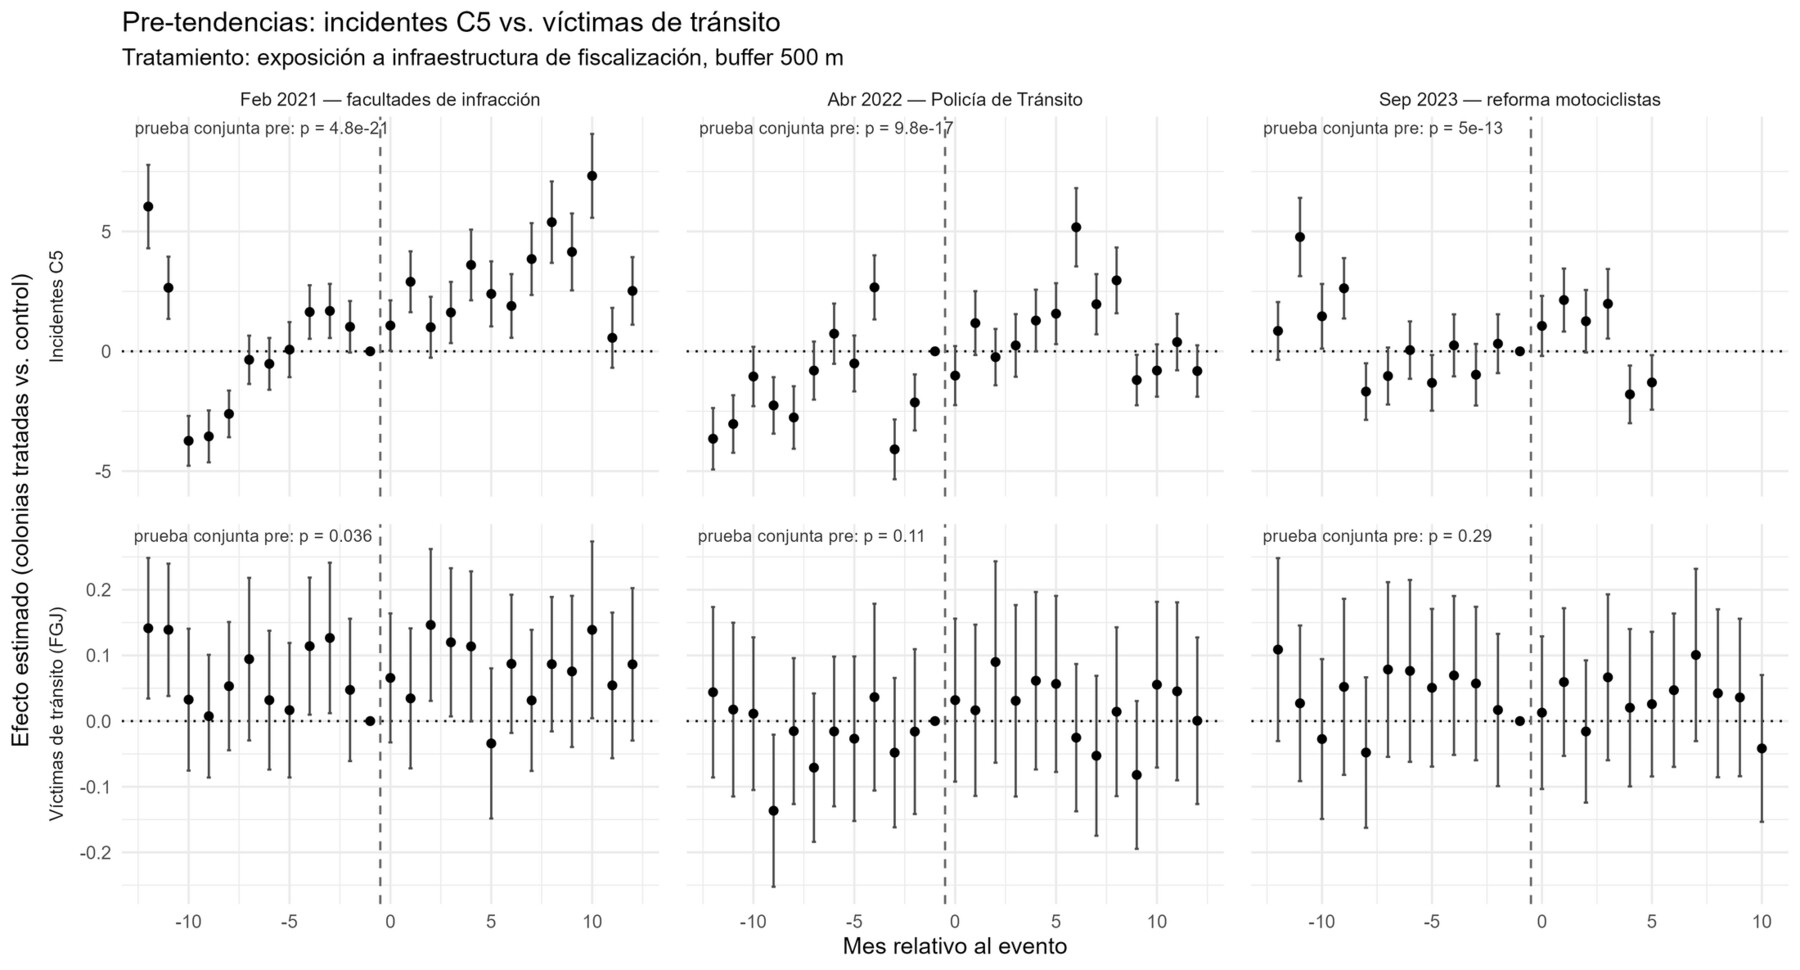
\includegraphics[width=\textwidth]{509_pretendencias_c5_vs_victimas.jpg}
  \caption{Estudio de evento para incidentes C5 (arriba) y víctimas de tránsito
  (abajo), en los tres cambios de política. \emph{buffer} de 500~m. En cada
  panel se anota el $p$-valor de la prueba conjunta de tendencias previas.}
  \label{fig:pretendencias}
\end{figure}

Con \textbf{incidentes C5} la prueba conjunta se rechaza en los tres eventos y en
todos los \emph{buffers} ($p \approx 10^{-16}$): las colonias cercanas a la
infraestructura vienen en una trayectoria creciente respecto a las lejanas, con
independencia del evento. Este \emph{outcome} no permite una interpretación
causal y se reserva como referencia secundaria.

Con \textbf{víctimas de tránsito} la prueba conjunta no se rechaza en abril de
2022 ni en septiembre de 2023 ($p = 0.11$ y $0.29$ respectivamente). El resto del
análisis se ancla en abril de 2022, el evento con primera etapa plausible
(Sección~\ref{sec:mecanismo}) y con más ventana posterior disponible.

\section{Efecto sobre las víctimas de tránsito}

La Figura~\ref{fig:victimas} presenta el estudio de evento de abril de 2022 para
el total de víctimas y para las víctimas fallecidas, en los tres \emph{buffers}.

\begin{figure}[H]
  \centering
  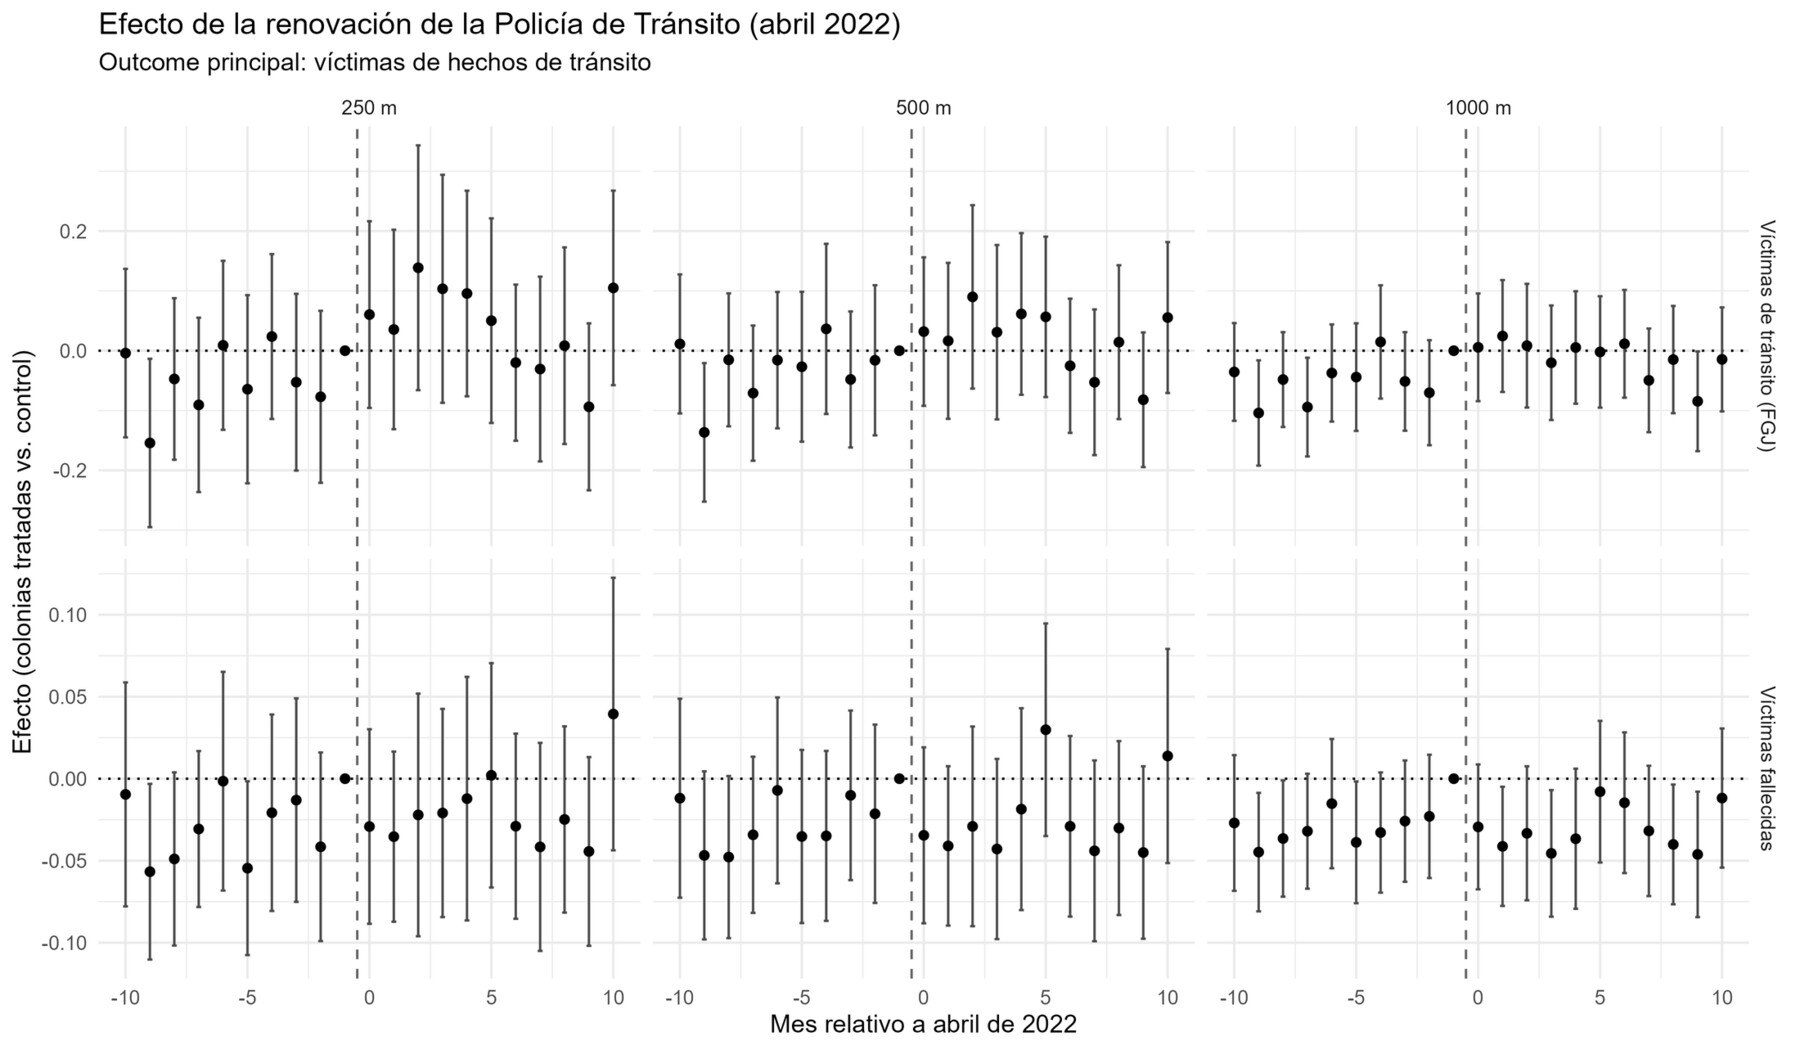
\includegraphics[width=\textwidth]{510_victimas.jpg}
  \caption{Estudio de evento de la renovación de la Policía de Tránsito
  (abril de 2022). \emph{Outcome}: víctimas de hechos de tránsito.}
  \label{fig:victimas}
\end{figure}

En el \emph{buffer} más estrecho (250~m) se observa un aumento transitorio del
total de víctimas en los primeros meses posteriores al evento, que se desvanece
hacia el mes $+6$. El efecto promedio posterior estimado por mínimos cuadrados
es de $+12$ a $+21\%$ según el \emph{buffer} (Tabla~\ref{tab:did}), marginalmente
significativo. Las \textbf{víctimas fallecidas no muestran ningún efecto} en
ninguna especificación ni horizonte.

\begin{table}[H]
  \centering
  \caption{Efecto promedio posterior (diferencia en diferencias agrupada),
  abril de 2022, ventana $-10/+10$.}
  \label{tab:did}
  \begin{tabular}{llrrr}
  \toprule
  \emph{Outcome} & \emph{buffer} & Efecto (\%) & $p$ & $p$ tend. previas \\
  \midrule
  Víctimas totales & 250 m  & $+21.5$ & 0.001 & 0.39 \\
  Víctimas totales & 500 m  & $+12.6$ & 0.03  & 0.17 \\
  Víctimas totales & 1000 m & $+11.8$ & 0.01  & 0.19 \\
  Víctimas fallecidas & 250 m  & $+14.8$ & 0.42 & 0.17 \\
  Víctimas fallecidas & 500 m  & $+0.7$  & 0.96 & 0.29 \\
  Víctimas fallecidas & 1000 m & $-7.6$  & 0.55 & 0.31 \\
  \bottomrule
  \end{tabular}
\end{table}

\clearpage
\section{Robustez}
\label{sec:robustez}

La Figura~\ref{fig:robustez} recopila el efecto promedio posterior bajo distintas
especificaciones: modelo lineal frente a Poisson de efectos fijos, tratamiento
binario frente a continuo, y ventanas previas alternativas.

\begin{figure}[H]
  \centering
  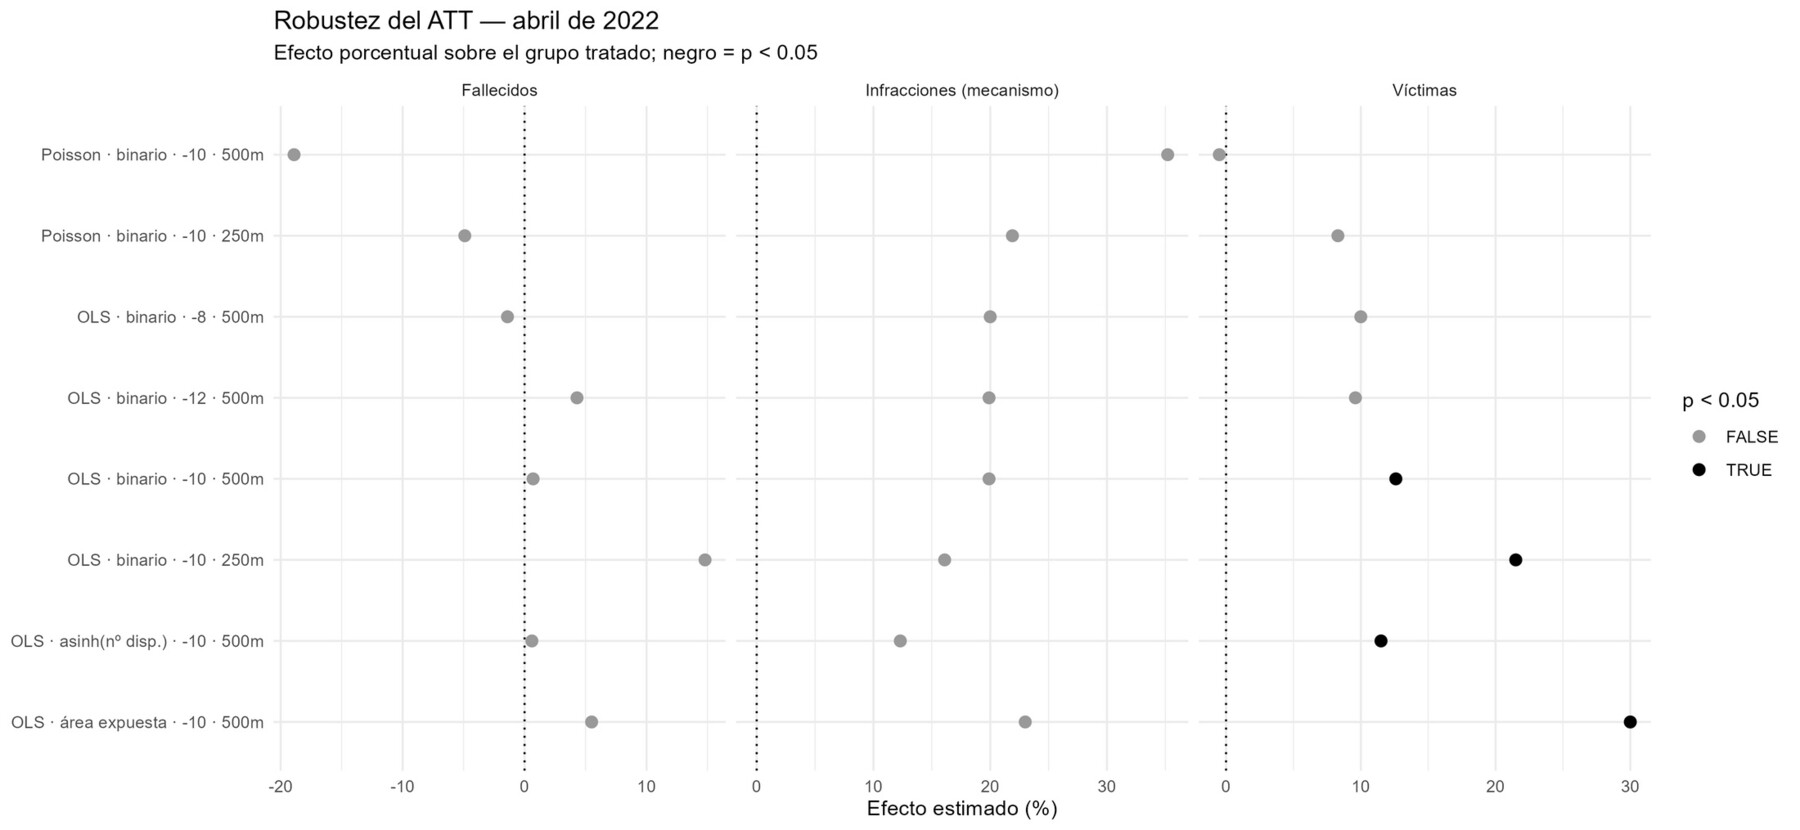
\includegraphics[width=\textwidth]{603_robustez_att.jpg}
  \caption{Robustez del efecto promedio posterior (abril de 2022). Puntos
  negros: $p<0.05$.}
  \label{fig:robustez}
\end{figure}

El resultado central es que \textbf{el efecto aparente sobre las víctimas totales
no es robusto}. Bajo un modelo de conteo (Poisson con efectos fijos de colonia y
mes), que es la especificación adecuada para un \emph{outcome} con 89\% de
observaciones en cero, el efecto desaparece ($-0.5\%$, $p = 0.93$ con
\emph{buffer} de 500~m; $+8\%$, $p = 0.22$ con 250~m). El efecto positivo que
aparece con mínimos cuadrados está impulsado por unas pocas colonias de vías
primarias con incrementos grandes en términos absolutos. Las víctimas fallecidas
permanecen sin efecto en todas las especificaciones.

\section{Mecanismo: fiscalización diferencial}
\label{sec:mecanismo}

La Figura~\ref{fig:mecanismo} muestra el estudio de evento de las infracciones
alrededor de abril de 2022.

\begin{figure}[H]
  \centering
  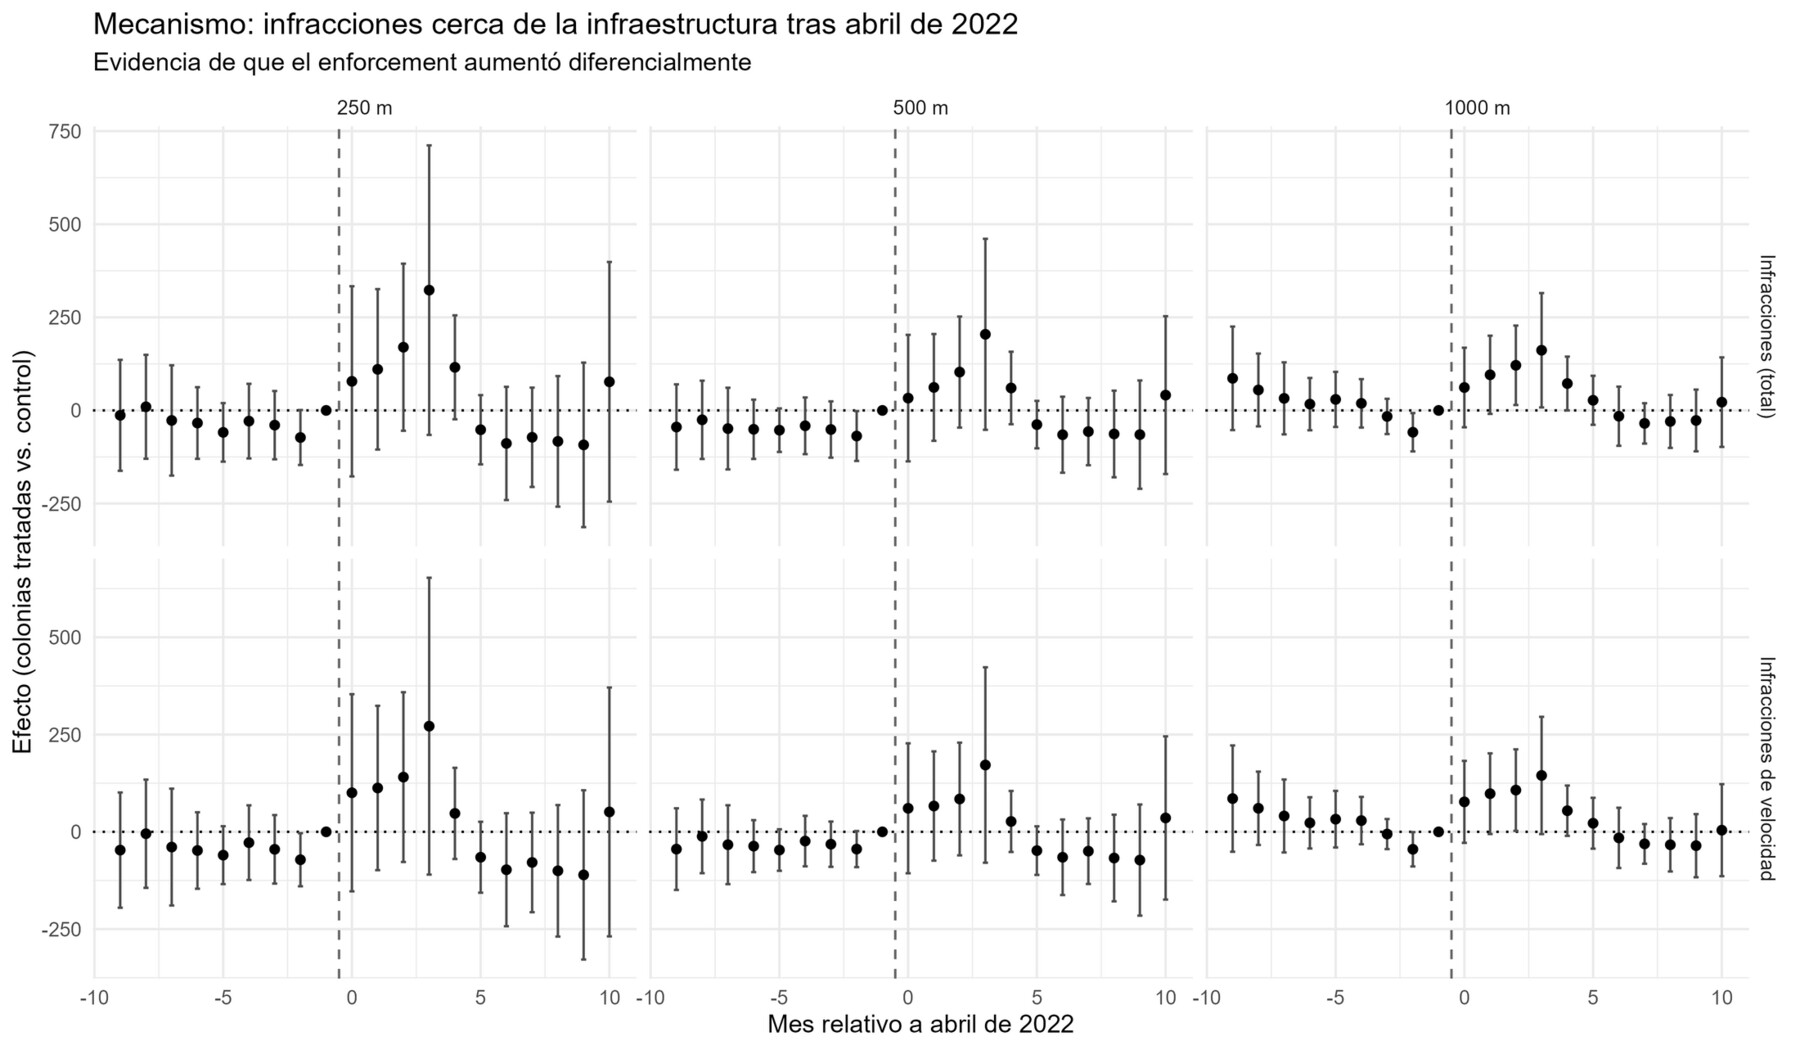
\includegraphics[width=\textwidth]{510_mecanismo_multas.jpg}
  \caption{Mecanismo: infracciones cerca de la infraestructura de fiscalización
  alrededor de abril de 2022.}
  \label{fig:mecanismo}
\end{figure}

Se observa un aumento transitorio de las infracciones cerca de la infraestructura
en los primeros meses posteriores a la reforma (del orden de $+15$ a $+35\%$ en
el estudio de evento para $k = 1,\dots,3$, más claro en el \emph{buffer} de
250~m), que regresa a su nivel base hacia el mes $+5$. El efecto promedio
posterior no es estadísticamente significativo ($p \approx 0.3$--$0.6$). La
evidencia de una fiscalización diferencial es, por tanto, \textbf{débil y de
corta duración}.

\section{Réplica en un segundo evento: septiembre de 2023}
\label{sec:replica_sep2023}

Para que la conclusión no dependa de un único cambio de política, se repite el
mismo diseño para la \textbf{reforma para motociclistas de septiembre de
2023}, evento que también cuenta con tendencias previas válidas para las
víctimas de tránsito (Sección~\ref{sec:pretendencias}). Se usa el inventario de
infraestructura de 2022 y la misma ventana $-10/+10$. No se estima el mecanismo
de infracciones: la fuente termina en abril de 2023, antes de este evento, por
lo que ni siquiera el mes de referencia cuenta con cobertura.

\begin{figure}[H]
  \centering
  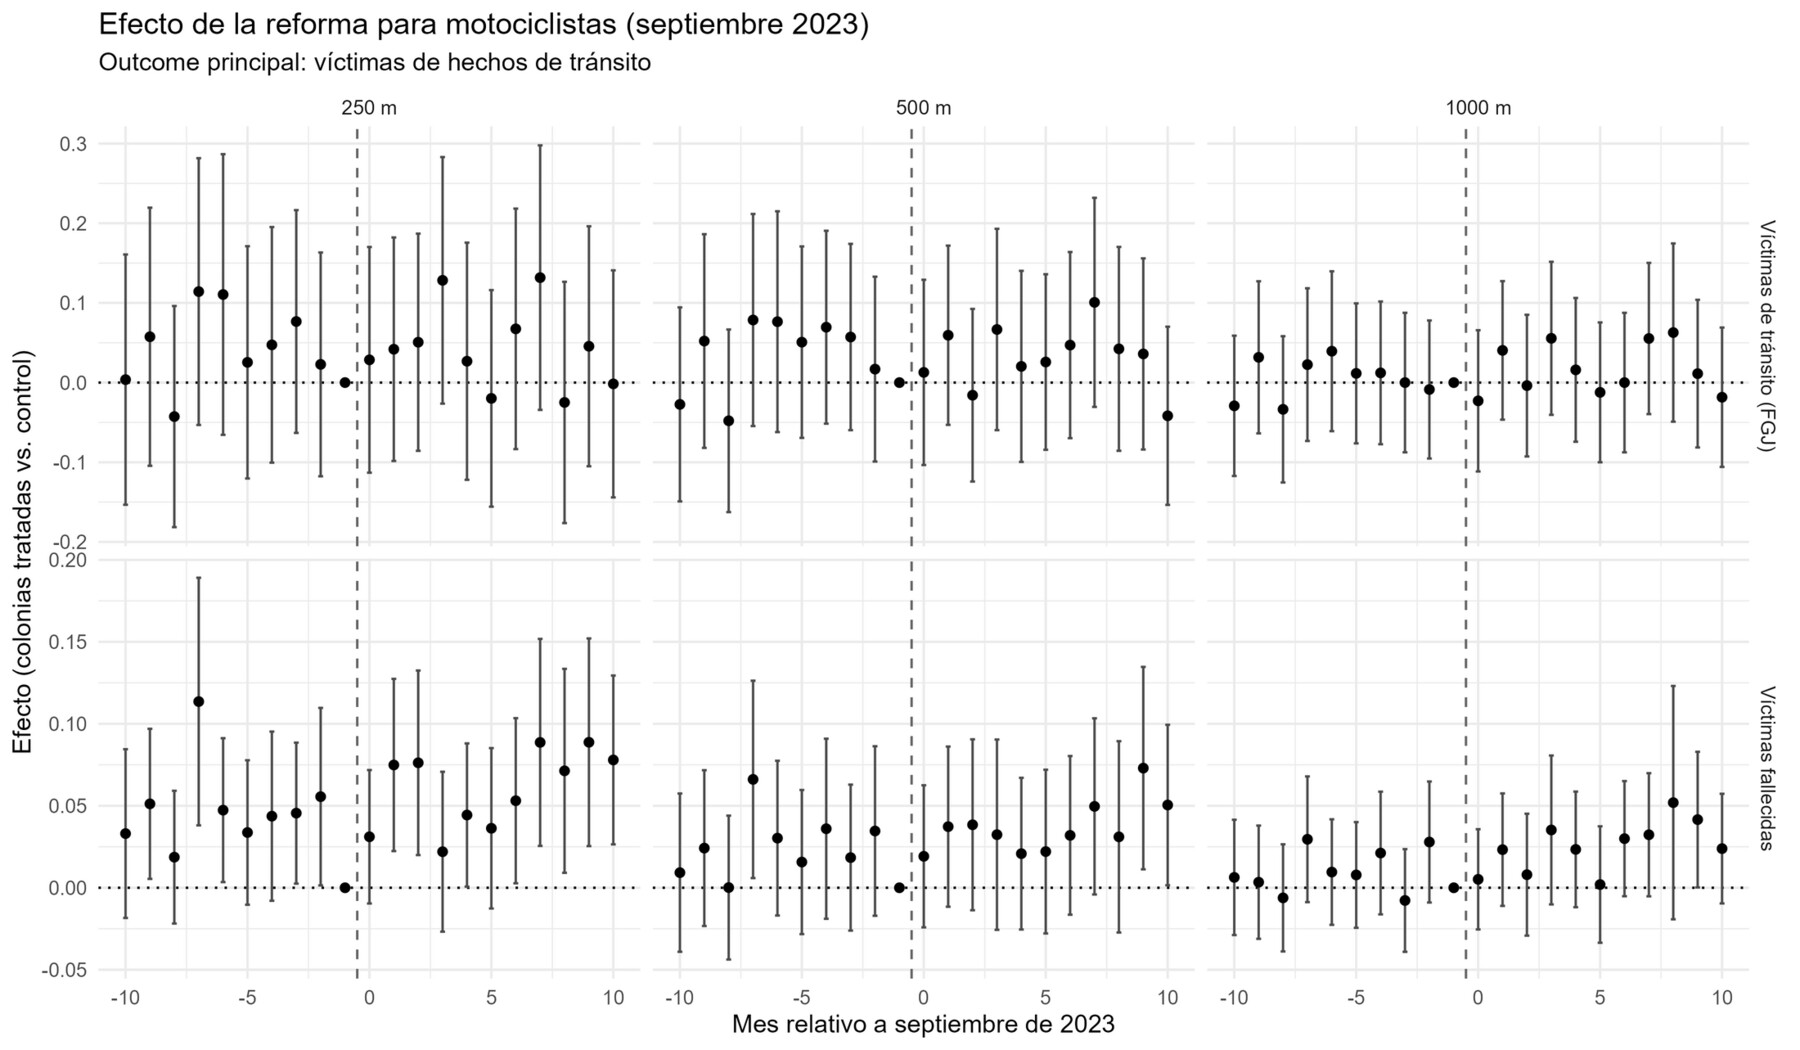
\includegraphics[width=\textwidth]{511_victimas.jpg}
  \caption{Estudio de evento de la reforma para motociclistas (septiembre de
  2023). \emph{Outcome}: víctimas de hechos de tránsito.}
  \label{fig:victimas_sep2023}
\end{figure}

\begin{figure}[H]
  \centering
  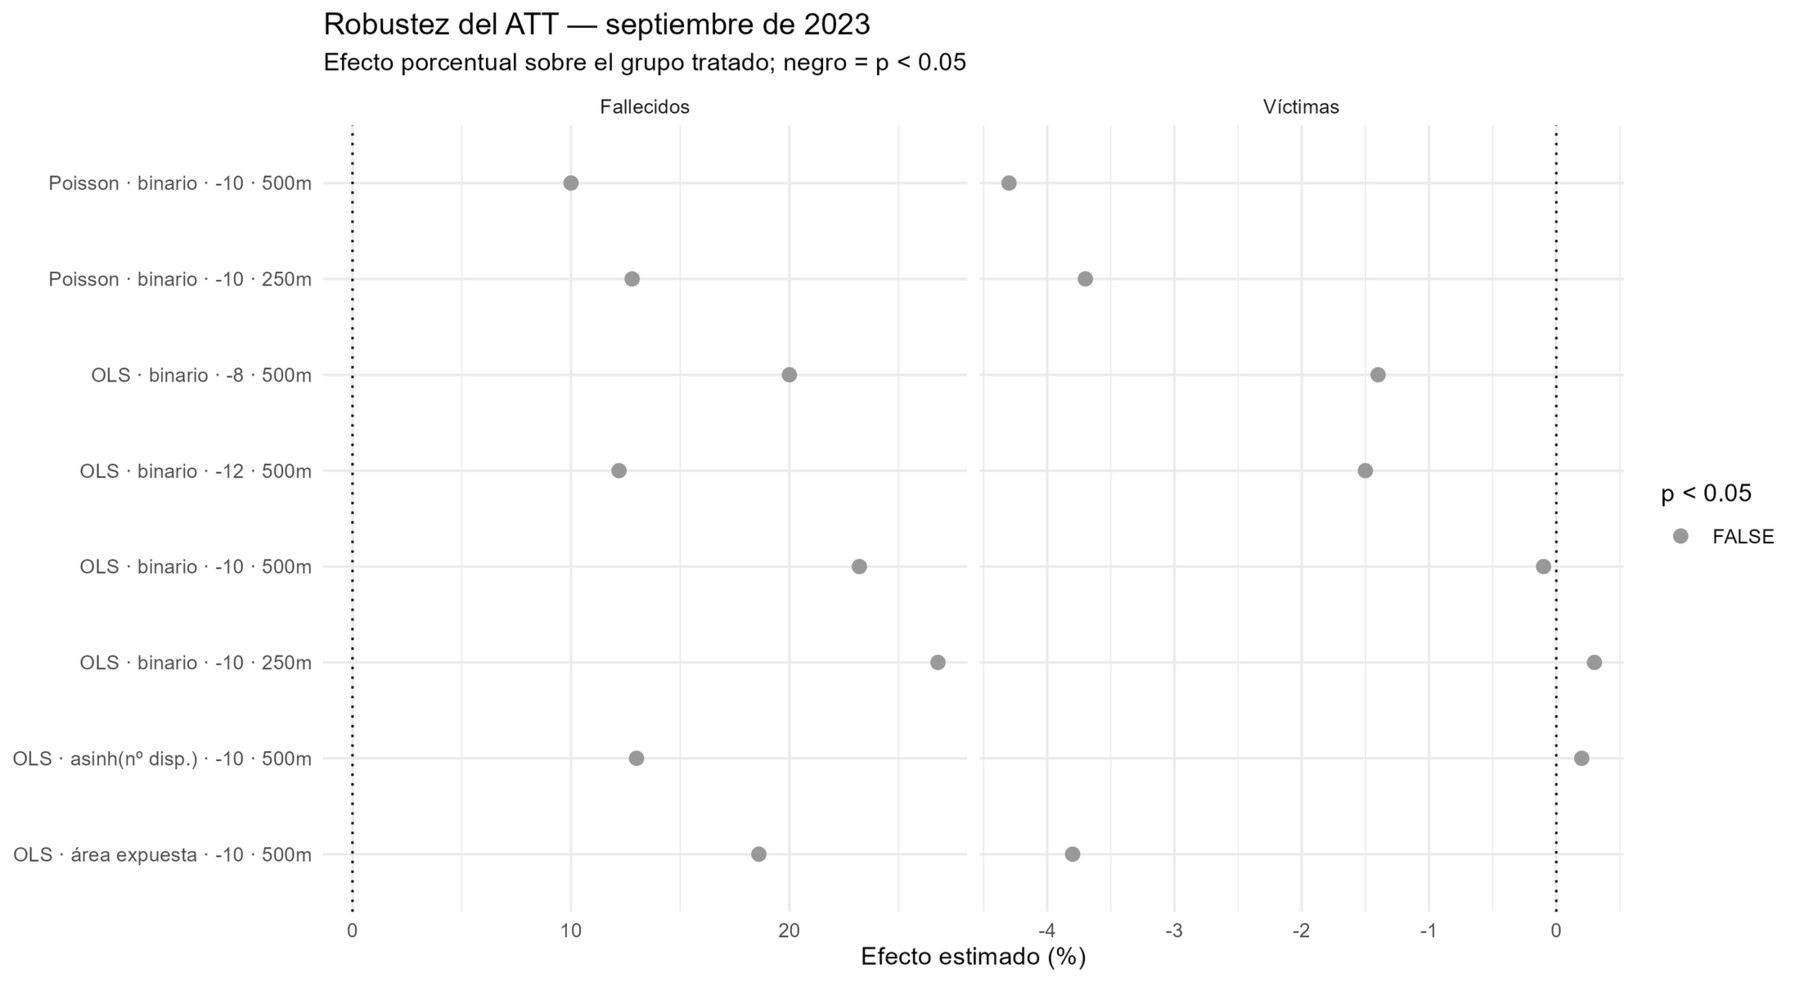
\includegraphics[width=0.85\textwidth]{604_robustez_att.jpg}
  \caption{Robustez del efecto promedio posterior, septiembre de 2023.}
  \label{fig:robustez_sep2023}
\end{figure}

El resultado es consistente con abril de 2022: las víctimas totales no muestran
efecto en ninguna especificación ($-4$ a $+4\%$, nunca significativo). Las
víctimas fallecidas muestran puntos estimados positivos bajo mínimos cuadrados
($+10$ a $+36\%$, marginalmente significativos en un par de especificaciones),
pero \textbf{ninguno sobrevive al modelo de conteo} ($p = 0.43$--$0.52$ con
Poisson). Los incidentes C5 vuelven a mostrar un rechazo fuerte de las
pre-tendencias y no se interpretan.

Que el resultado nulo se repita en dos eventos distintos —con mecanismos
institucionales diferentes y separados por año y medio— hace más creíble que la
ausencia de efecto no es una particularidad de abril de 2022.

\section{Síntesis}

No se encuentra evidencia robusta de que la renovación de la Policía de Tránsito
de abril de 2022 haya reducido las víctimas de hechos de tránsito en las zonas
con infraestructura de fiscalización. Las víctimas fallecidas no cambian en
ninguna especificación; el aumento aparente en víctimas totales no sobrevive a un
modelo de conteo y coincide en momento y duración con el repunte transitorio de
las infracciones, lo que sugiere un efecto de reporte más que un deterioro real
de la seguridad vial. La propia intervención —una fiscalización diferencial
inducida por la reforma— es débil y transitoria, por lo que el resultado nulo
debe leerse como ausencia de evidencia de efecto en un contexto donde el
tratamiento es en sí mismo tenue, más que como un cero estimado con precisión.

La réplica en septiembre de 2023 (Sección~\ref{sec:replica_sep2023}) refuerza
esta lectura: en un evento distinto, con otro mecanismo institucional, el mismo
diseño vuelve a arrojar un nulo robusto una vez que se controla adecuadamente la
dispersión del conteo de víctimas. La ausencia de efecto no parece, entonces,
una particularidad de un solo cambio de política.

\chapter{Conclusiones}
\label{chap:conclusiones}

\noindent
Este trabajo evaluó si el aumento de la fiscalización vial asociado a la
renovación de la Policía de Tránsito de la Ciudad de México (abril de 2022)
redujo las víctimas de hechos de tránsito, comparando la evolución de las
colonias expuestas a la infraestructura de fiscalización con la de las no
expuestas.

No se encuentra evidencia robusta de un efecto. Las víctimas fallecidas —el
\emph{outcome} menos sensible a los efectos de reporte— no cambian en ninguna
especificación. El aumento aparente en las víctimas totales bajo mínimos
cuadrados no sobrevive a un modelo de conteo y coincide en momento y duración
con un repunte transitorio de las infracciones, lo que sugiere un efecto de
registro más que un cambio real en la siniestralidad.

\section{Cómo leer el nulo}

Un resultado nulo admite al menos dos lecturas, y conviene ser explícito sobre
cuál corresponde a este trabajo. La primera es que la fiscalización vial, bien
implementada, no tiene capacidad de reducir víctimas de tránsito —un hallazgo
fuerte, y de alguna forma sorprendente a la luz de \citet{deangelohansen2014},
quien sí encuentra un efecto grande del enforcement policial sobre la
mortalidad vial en su contexto—. La segunda, más modesta y más consistente
con la evidencia reunida aquí, es que \emph{esta} intervención en particular
—la renovación de la Policía de Tránsito— no generó una fiscalización
diferencial lo bastante fuerte ni lo bastante sostenida como para mover el
outcome, independientemente de si el mecanismo funcionaría con una
intervención de mayor intensidad. El mecanismo (Sección~\ref{sec:mecanismo})
muestra un incremento de apenas 10 a 35\,\% en infracciones cerca de la
infraestructura, nunca estadísticamente significativo de forma individual, y
concentrado en una ventana de aproximadamente cuatro meses antes de disiparse.
Un primer paso tan débil deja poco margen para observar un efecto en el
segundo. El nulo de esta tesis debe leerse, entonces, como \emph{ausencia de
evidencia de un efecto bajo un tratamiento débil}, y no como una estimación
precisa de un efecto verdaderamente cero. La réplica en septiembre de 2023
(Sección~\ref{sec:replica_sep2023}) refuerza la robustez del patrón —el mismo
nulo aparece en un segundo evento, con otra reforma y otra infraestructura de
referencia— pero no resuelve esta ambigüedad de fondo, porque tampoco en ese
caso hay evidencia de una fiscalización diferencial fuerte.

\section{Relación con la versión previa de esta investigación}

La versión anterior de este proyecto estimaba, con un diseño de variables
instrumentales a nivel código postal, que un mayor volumen de multas se
asociaba con \emph{más} accidentes de tránsito. El instrumento —haber
recibido infracciones por encima de la mediana en el periodo previo— no
satisfacía de forma creíble la restricción de exclusión: es difícil sostener
que el historial de multas de una zona afecta la accidentalidad únicamente a
través de las multas contemporáneas, y no a través de características de la
zona (tipo de vialidad, volumen de tráfico, comportamiento de los
conductores) correlacionadas con ambas variables. El rediseño que da lugar a
esta tesis corrige tres decisiones de ese diseño original: cambia la unidad de
análisis de código postal a colonia, que es la unidad administrativa sobre la
que efectivamente varía la infraestructura de fiscalización; abandona el
enfoque de variables instrumentales en favor de un estudio de evento con
efectos fijos, sin pretender resolver la endogeneidad de las multas por la vía
de un instrumento débil; y trata las multas explícitamente como
\emph{mecanismo} —evidencia de que hubo más fiscalización— en vez de como la
variable de interés central, desplazando esa posición a las víctimas de
tránsito. El resultado cambia en consecuencia: de un efecto positivo y
significativo, pero apoyado en un instrumento cuestionable, a un nulo robusto
a la especificación, apoyado en una fuente de variación más transparente
—dónde se ubica la infraestructura de fiscalización— aunque también más
débil.

\section{Implicaciones y trabajo futuro}

Con las salvedades del nulo señaladas arriba, este trabajo deja tres
implicaciones. Primero, una reforma institucional de la policía de tránsito
—cambiar quién puede infraccionar y cómo, sin necesariamente ampliar de forma
sostenida la infraestructura física de fiscalización— no es, por sí sola,
garantía de una fiscalización diferencial fuerte; el mecanismo de esta tesis
lo muestra de forma directa. Segundo, los efectos de reporte son un reto
central, y con frecuencia subestimado, para evaluar políticas de seguridad
vial con datos administrativos: el hecho de que el efecto aparente sobre
víctimas totales desaparezca al usar fallecidos —y de que ambos coincidan en
tiempo con el repunte de multas— es exactamente el patrón que produciría un
cambio en la probabilidad de registro sin un cambio real en la
siniestralidad, y cualquier evaluación de este tipo de política debería
distinguir explícitamente entre ambos canales, como se hace aquí
(Sección~\ref{sec:contexto_espacial}). Tercero, la literatura de disuasión
policial \citep{chalfinmccrary2017,deangelohansen2014} sugiere que
el margen relevante no es solo la fiscalización, sino su intensidad y su
persistencia; un análisis que solo observe si hubo o no una reforma, sin
medir directamente cuánto cambió la fiscalización efectiva, corre el riesgo de
atribuir a la política un efecto —o una ausencia de efecto— que en realidad
depende de qué tan bien se implementó.

Quedan al menos tres líneas de trabajo futuro. La más directa es cambiar la
unidad de análisis de colonia a segmento vial, lo que permitiría una
definición de exposición más precisa que un buffer de distancia y reduciría
el problema de que la infraestructura y la siniestralidad comparten
determinantes a nivel colonia (Sección~\ref{sec:datos_descriptivos}). Una
segunda línea es construir un grupo de control por \emph{matching} explícito
sobre las características previas al evento, en vez de depender enteramente
de los efectos fijos para absorber la diferencia de niveles entre colonias
tratadas y no tratadas. Una tercera es extender la ventana posterior del
análisis conforme se actualicen las fuentes de datos —en particular, C5 más
allá de febrero de 2024 e infracciones más allá de abril de 2023— lo que
permitiría evaluar con outcome de mecanismo eventos más recientes, como la
propia reforma de motociclistas de septiembre de 2023, que en esta tesis solo
pudo replicarse para el outcome de víctimas.


%------------------------------------------------------------------------------
%  BIBLIOGRAFÍA
%------------------------------------------------------------------------------
\chapter*{Referencias}
\addcontentsline{toc}{chapter}{Referencias}
\bibliographystyle{apalike}
\bibliography{referencias/ref}

\end{document}
